\section{Experiments}
\label{sec:experiments}

% one point to discuss about teher length, extends operaion.
% dsicussion on how to define maximum tether length to entaglement.
% What is the common operational tether length in industry? 
%cost benefit analysis for tether saving vs time saving

% when comaping planner compare them relative to each other percentage

% Mention that after inspection, we need to deantgale so this will take time for CPP 

%Mention that this scaled model sceanrio 

%
%Offline vs online discussion
%

%online allows for arbitrary fixation.

% allows for suggestion for remotely 

% can be emebeded in offline planer

% Run one more shape for simulations.

% Add detangeling operaton.


% Arguments to add to discussion why our online planner is very good.
% 1. Online planning allows for dynamic adaptaion even if the trajetcory followed is not the same, or the environment changes (more robust and adaptive).
% 2. Comp

This section presents the experimental results of our proposed \ac{REACT} method. The entire framework is implemented in C++ to ensure computational efficiency, and integrated with ROS to facilitate modularity and ease of deployment on real-world robotic systems. For the planning component, we utilize the \ac{OMPL} library \cite{ompl} to compute shortest paths using the RRT* algorithm.  


\subsection{Experimental Set Up}
The path planner is implemented for a BlueROV2. A \ac{MPC} approach is chosen to account for model constraints and to provide the optimal control input $\mathbf{u}^{ref} \in \mathbb{R}^4$, where $\mathbf{u}^{ref} = [F_x, F_y, F_z, M_z]^T$ represents the forces in the $X$, $Y$, and $Z$ directions, and the moment about the $Z$-axis. The goal is to follow the desired reference trajectory $\mathbf{x}^{ref} \in \mathbb{R}^6$, where $\mathbf{x}^{ref} = [x_{ref}, y_{ref}, z_{ref}, \psi_{ref}]^T$ contains the reference position ($x_{ref}$, $y_{ref}$, $z_{ref}$) and the reference yaw angle $\psi_{ref}$.

The entanglement-aware path planner provides $\mathbf{x}^{ref}$ in real time, ensuring the BlueROV2 avoids obstacles while following the desired trajectory. For further details about the controller and model, the reader is referred to \cite{amergp}.

%\subsection{Results}
We perform a comparative analysis of the proposed \ac{REACT} method and a baseline conventional \ac{CPP} (FC-Planner \cite{feng2024fc}), which does not contain explicit entanglement handling. 

The simulation setup consists of a pipe structure represented by an underwater pipe model from \cite{feng2024fc}. The simulated onboard camera featured a horizontal field of view of 70 degrees and a vertical field of view of 60 degrees, with a maximum inspection range of 3.0 meters. The tether constraint was defined by a maximum allowable tether length of $L_{max}$ = 10.0 meters.

Environmental coverage was evaluated geometrically similar to \cite{amer2023visual}. At each subsampled time step, the position and orientation of the camera were used to determine which triangles in the environment mesh were visible. A triangle was marked as visible if its centroid was within the inspection range, its surface normal faced the camera, and its projection lay within the camera's field of view. Over time, the set of all uniquely observed triangles was accumulated. The coverage at time $t$ was defined as the ratio of the number of unique visible triangles up to time $t$ to the total number of triangles in the environment.


\subsection{Results}

The quantitative performance metrics for both planners are summarized in Table~\ref{tab:performance_metrics}.

\begin{table}[ht]
    \centering
    \caption{Performance Metrics Comparison}
    \label{tab:performance_metrics}
    \resizebox{0.8\columnwidth}{!}{%
    \begin{tabular}{|l|c|c|c|}
        \hline
        \textbf{Planner} & \textbf{Total Time (s)}  & \textbf{Final Coverage (\%)} \\
        \hline
        \ac{REACT} & 546.00  & 99.91 \\
        CPP  & 429.00  & 99.82 \\
        \hline
    \end{tabular}%
    }
    \vspace{0.5em}
\end{table}


Figures~\ref{fig:coverage_vs_time} and~\ref{fig:tether_vs_time} visualize the performance of the planners in terms of environmental coverage and tether length, respectively.

\begin{figure}[ht]
    \centering
    \begin{subfigure}[b]{0.48\linewidth}
        \centering
        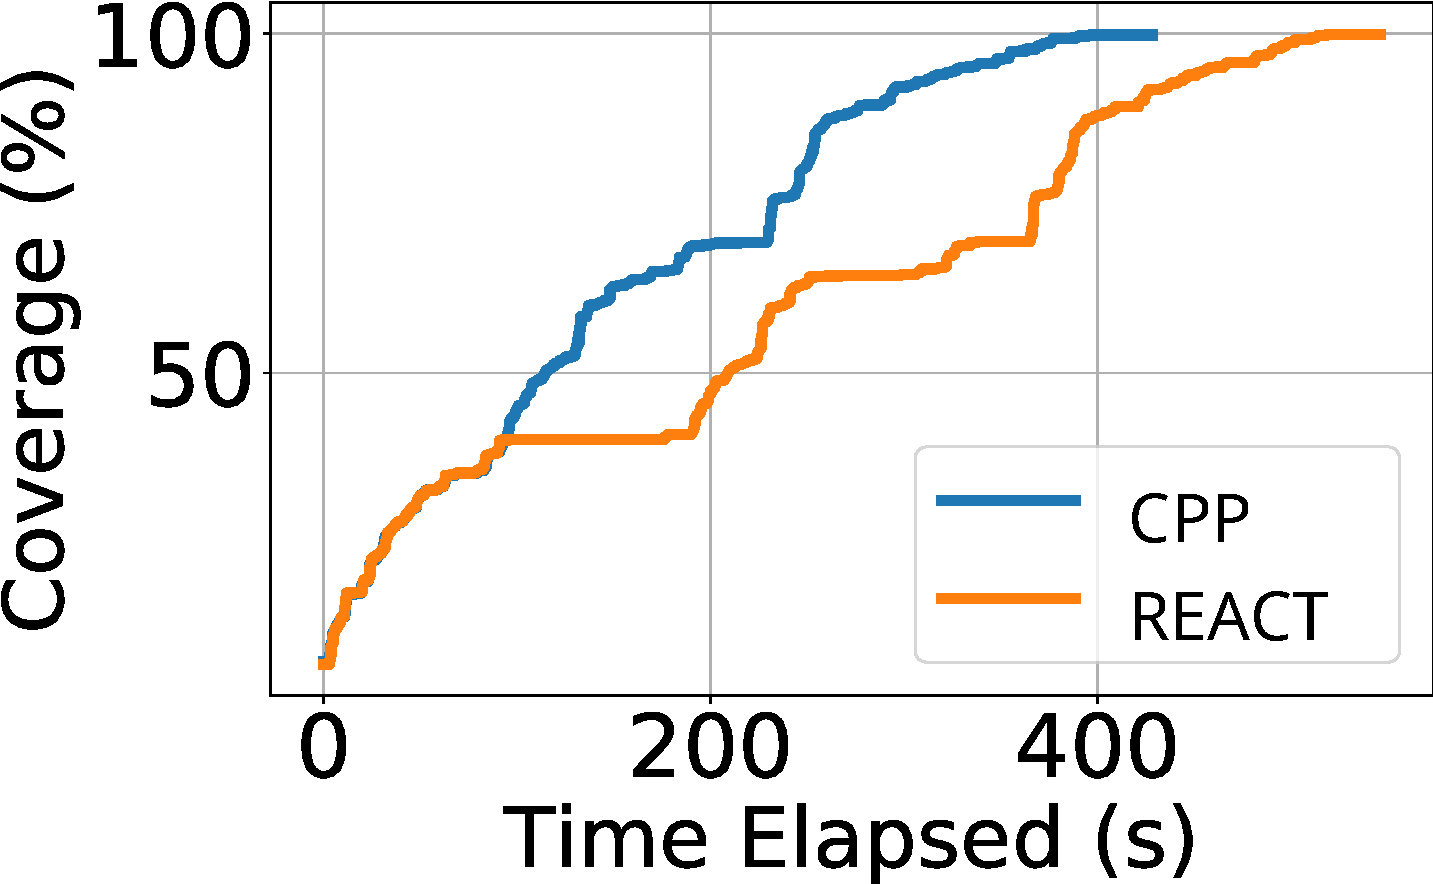
\includegraphics[width=\linewidth]{coverage_vs_time.pdf}
        \caption{Environmental Coverage vs. Time for both planners.}
        \label{fig:coverage_vs_time}
    \end{subfigure}
    \hfill
    \begin{subfigure}[b]{0.48\linewidth}
        \centering
        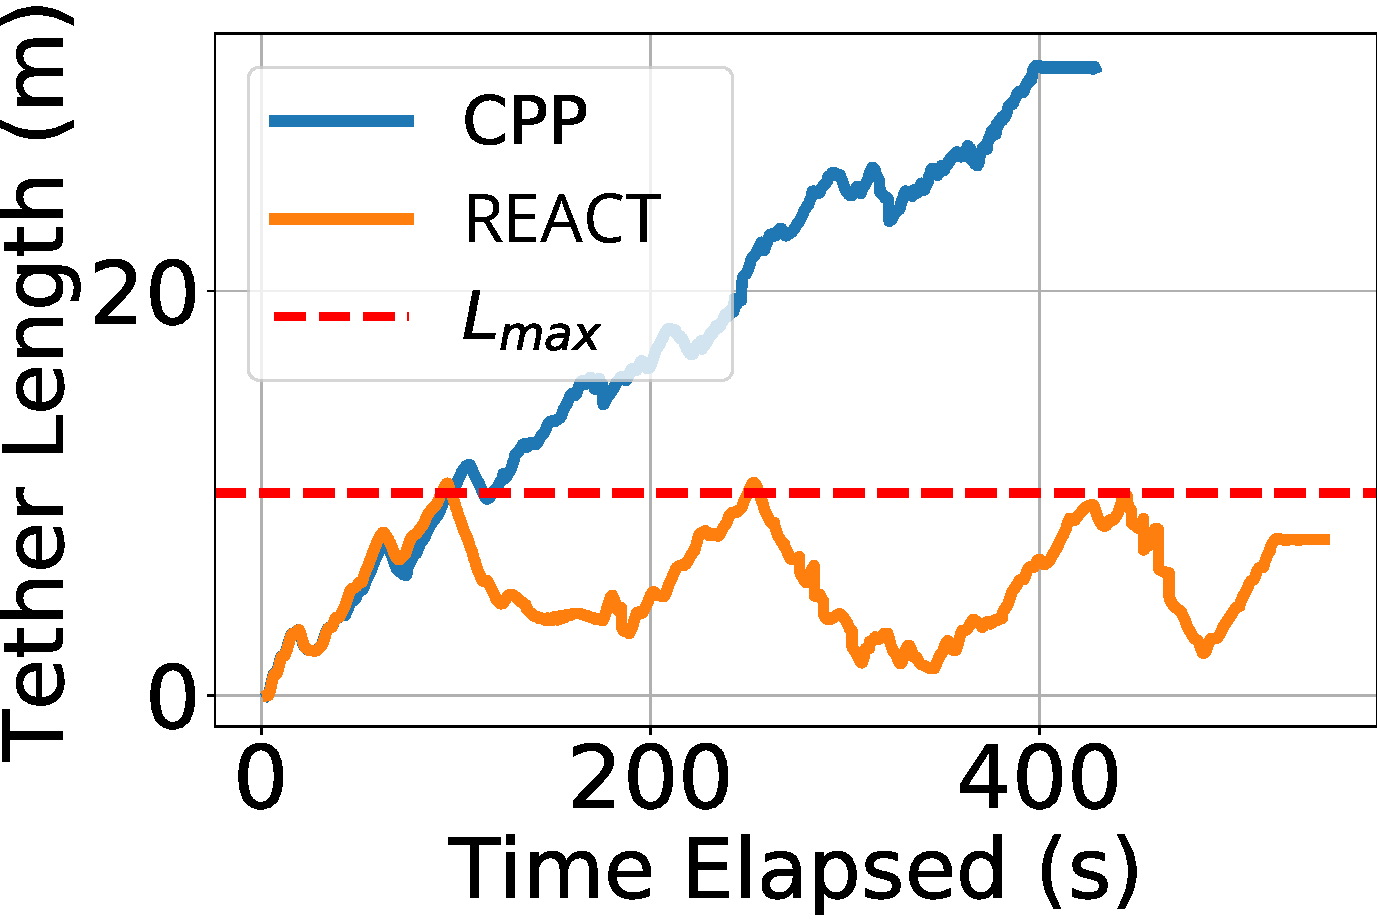
\includegraphics[width=\linewidth]{tether_length_vs_time.pdf}
        \caption{Tether Length vs. Time, highlighting the 10.0m maximum limit.}
        \label{fig:tether_vs_time}
    \end{subfigure}
    \caption{Comparison of coverage and tether behavior over time.}
    \label{fig:coverage_tether_sidebyside}
\end{figure}


\begin{figure}[ht]
    \centering
    \begin{subfigure}[b]{0.48\linewidth}
        \centering
        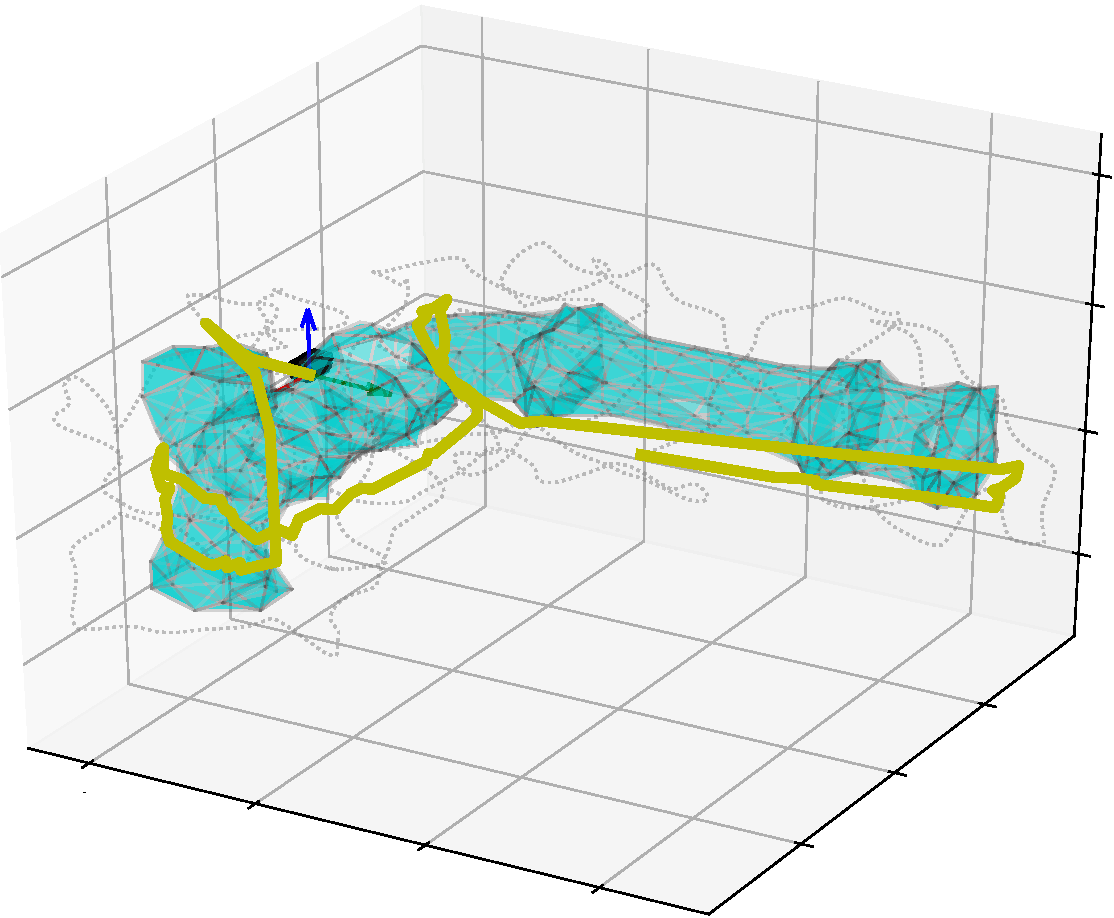
\includegraphics[width=\linewidth]{EA-Planner/figures/fc_planner_final_view.pdf}
        \caption{3-D plot CPP.}
        \label{fig:3d_cpp}
    \end{subfigure}
    \hfill
    \begin{subfigure}[b]{0.48\linewidth}
        \centering
        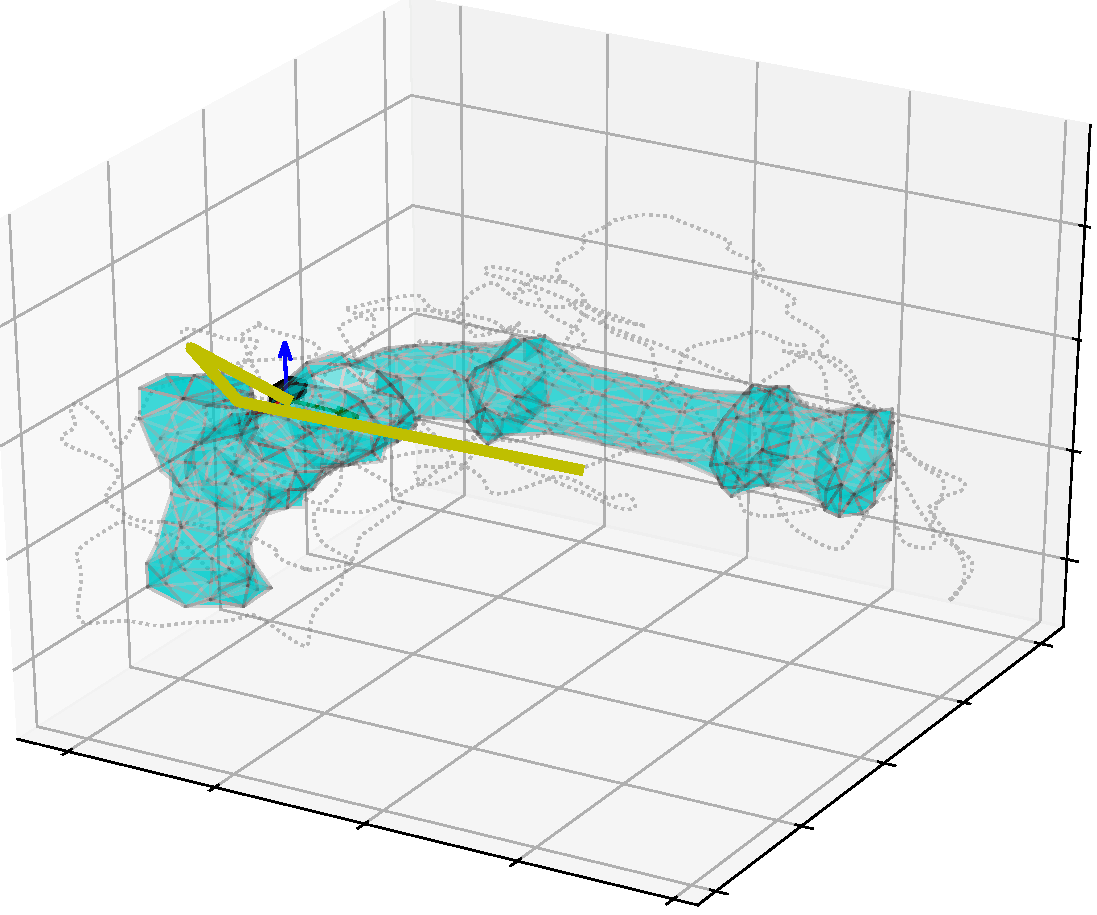
\includegraphics[width=\linewidth]{EA-Planner/figures/react_pipe.pdf}
        \caption{3-D plot, \ac{REACT}.}
        \label{fig:3d_oea}
    \end{subfigure}
    \caption{3D views of final trajectories. (a) CPP results in entangled tether geometry. (b) \ac{REACT} yields a non-entangled tether configuration, reflecting effective entanglement avoidance.}
    \label{fig:3Dplots}
\end{figure}




The results highlight distinct trade-offs between the two planning strategies. The \ac{CPP}, lacking entanglement awareness, completed the trajectory significantly faster (429.00~s vs. 546.00~s) while achieving marginally less final coverage (99.81\% vs. 99.91\%).

However, focusing solely on speed and final coverage overlooks the critical aspect of tether management in constrained environments. As shown in Figure~\ref{fig:tether_vs_time},\ac{CPP} planner exceeded the $L_{\text{max}}$ constraint during execution. 

This metric requires careful interpretation. \ac{REACT} is explicitly designed to avoid and react to potential tether entanglement. Its reactive replanning often involves maneuvers specifically intended to reposition the \ac{ROV} and adjust the tether configuration for safety. These maneuvers can temporarily increase tether length, potentially causing earlier—but controlled and intentional—exceedances of the simple length threshold as the planner actively works to prevent more critical entanglement states later in the mission.

Conversely, the \ac{CPP}, lacking this foresight and reactivity, proceeds along its path until physical constraints force a violation. While this happened slightly later in this simulation, the approach risks encountering more severe or unrecoverable tether states without the ability to proactively mitigate them.

The longer execution time of the \ac{REACT} directly reflects the computational cost of tether modeling, collision checking for the tether, and executing reactive replanning maneuvers when necessary. This deliberate approach prioritizes tether safety and mission robustness over raw speed, offering a significant advantage for reliable operation in complex, real-world underwater scenarios where tether integrity is paramount. 

The \ac{CPP}'s speed advantage comes at the cost of ignoring potential tether hazards, making it less suitable for missions where entanglement poses a significant risk. Therefore, \ac{REACT} demonstrates superior performance in the context of safe and robust tethered \ac{ROV} operation, despite the longer completion time observed in this comparison.












